\section{Sequence Diagrams}
\label{sec:sequencediagrams}
To complement the class diagram, this section presents sequence diagrams for key IoT-REAP workflows: VM session provisioning and termination, camera control, user authentication, and training unit progression. These diagrams illustrate interactions between Controllers, Services, external APIs (Proxmox, Guacamole, MQTT broker), and frontend Views, linking the system architecture to its implementation in Chapter~\ref{chap:realization}.

\newpage
\vspace{-1.3em}
\subsection{Manage Session Sequence}
\vspace{-0.7em}

Figure~\ref{fig:seq-manage-session} illustrates the manage session sequence.
\vspace{-0.7em}

\begin{figure}[H]
    \centering
    \includegraphics[width=0.9\textwidth]{assets/chapter2/Sequence-Manage-Session}
    \caption{Sequence Diagram: Manage Session}
    \label{fig:seq-manage-session}
\end{figure}

\newpage

\subsection{Discover Gateway Node Sequence}
Figure~\ref{fig:seq-discover-gateway} illustrates the discover gateway node sequence.
\begin{figure}[H]
    \centering
    \includegraphics[width=\textwidth]{assets/chapter2/Sequence-Discover-Gateway-Node}
    \caption{Sequence Diagram: Discover Gateway Node}
    \label{fig:seq-discover-gateway}
\end{figure}
\newpage

\subsection{Payout Request Sequence}
Figure~\ref{fig:seq-payout-request} illustrates the payout request sequence.
\begin{figure}[H]
    \centering
    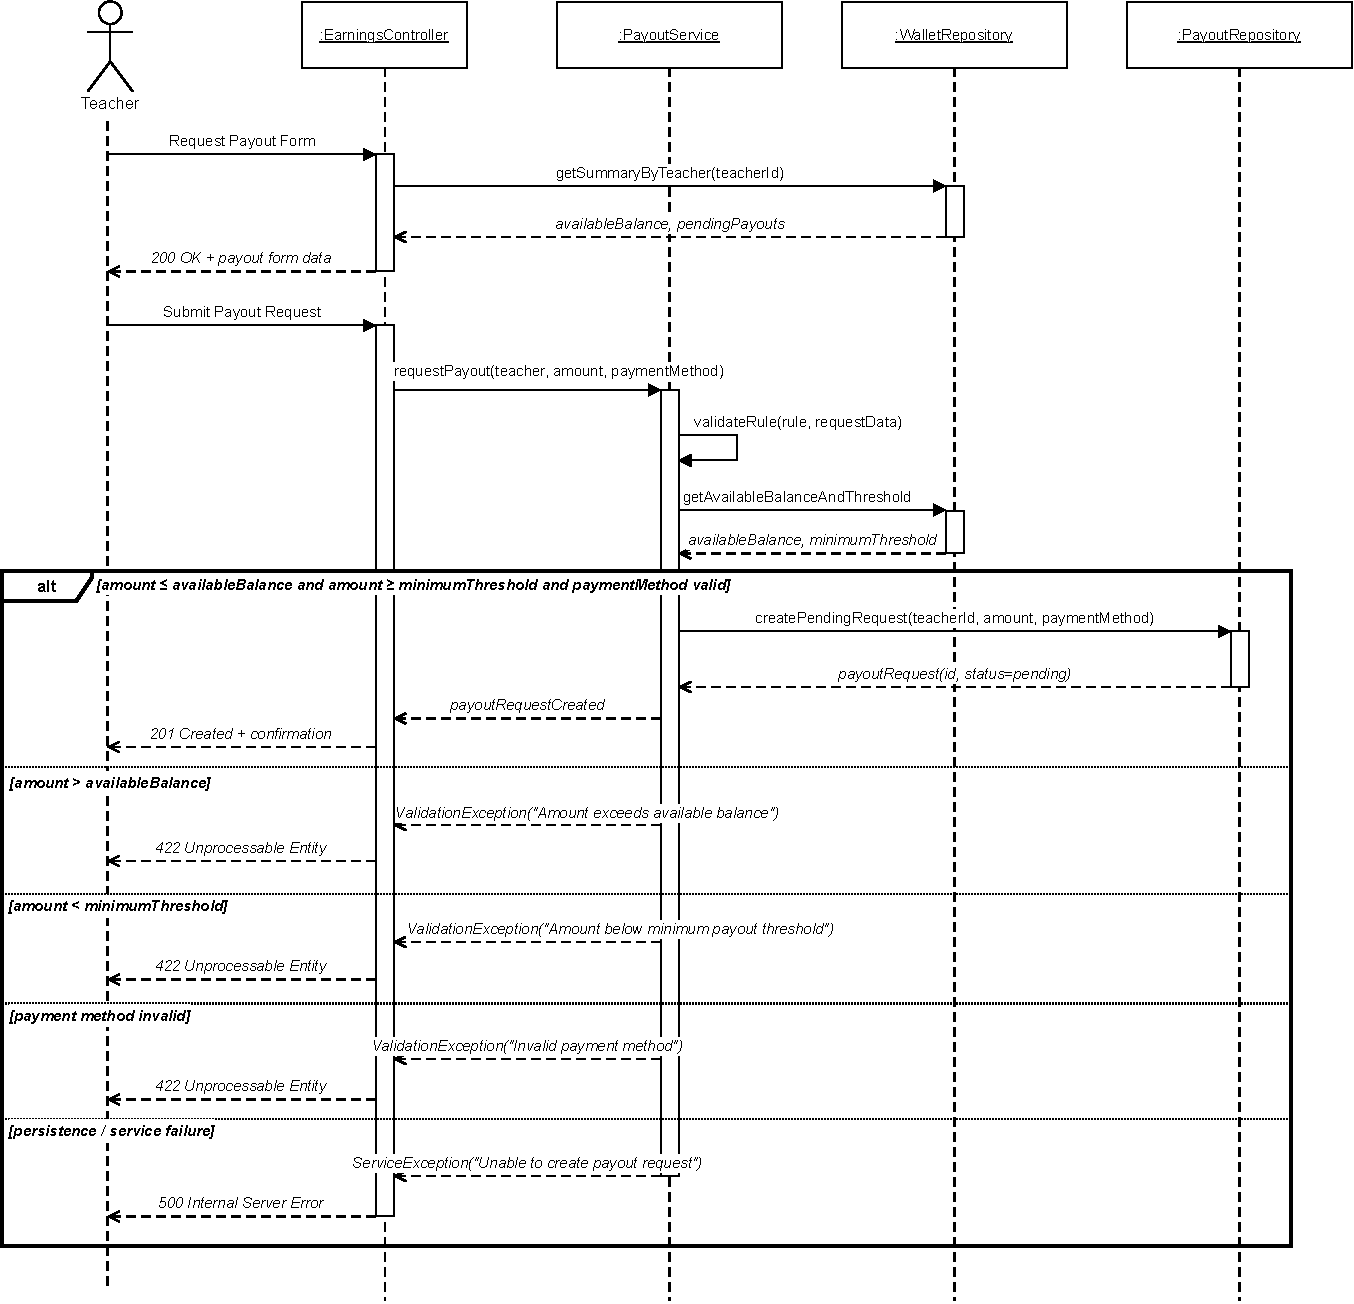
\includegraphics[width=\textwidth]{assets/chapter2/Sequence-Request-Payout}
    \caption{Sequence Diagram: Payout Request}
    \label{fig:seq-payout-request}
\end{figure}
\newpage
\vspace{-0.7em}
\subsection{Provision VM Session Sequence}
\vspace{-0.7em}
Figure~\ref{fig:seq-provision-vm-session} illustrates the provision VM session sequence.
\vspace{-0.7em}

\begin{figure}[H]
    \centering
    \rotatebox{90}{
        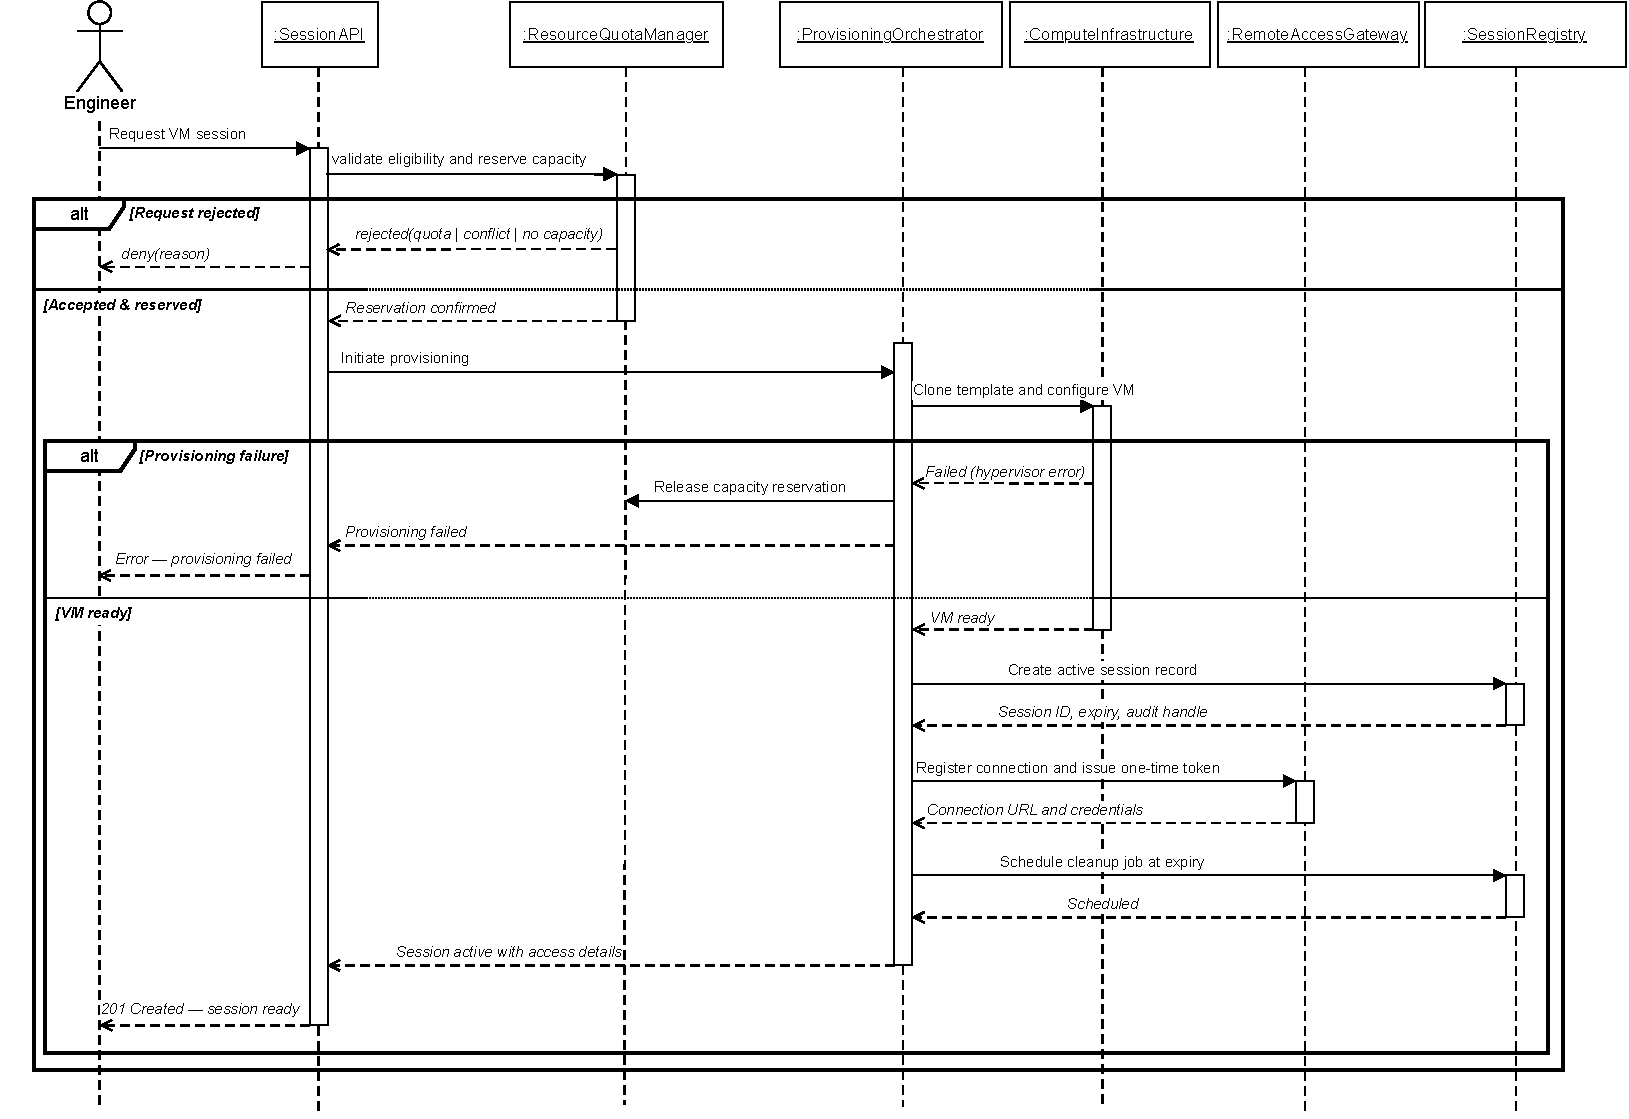
\includegraphics[height=\textwidth]{assets/chapter2/sequence-Provision-VM-Session}
    }
    \caption{Sequence Diagram: Provision VM Session}
    \label{fig:seq-provision-vm-session}
\end{figure}
\newpage

\subsection{User Authentication Sequence}
Figure~\ref{fig:seq-user-authentication} illustrates the user authentication sequence.
\begin{figure}[H]
    \centering
    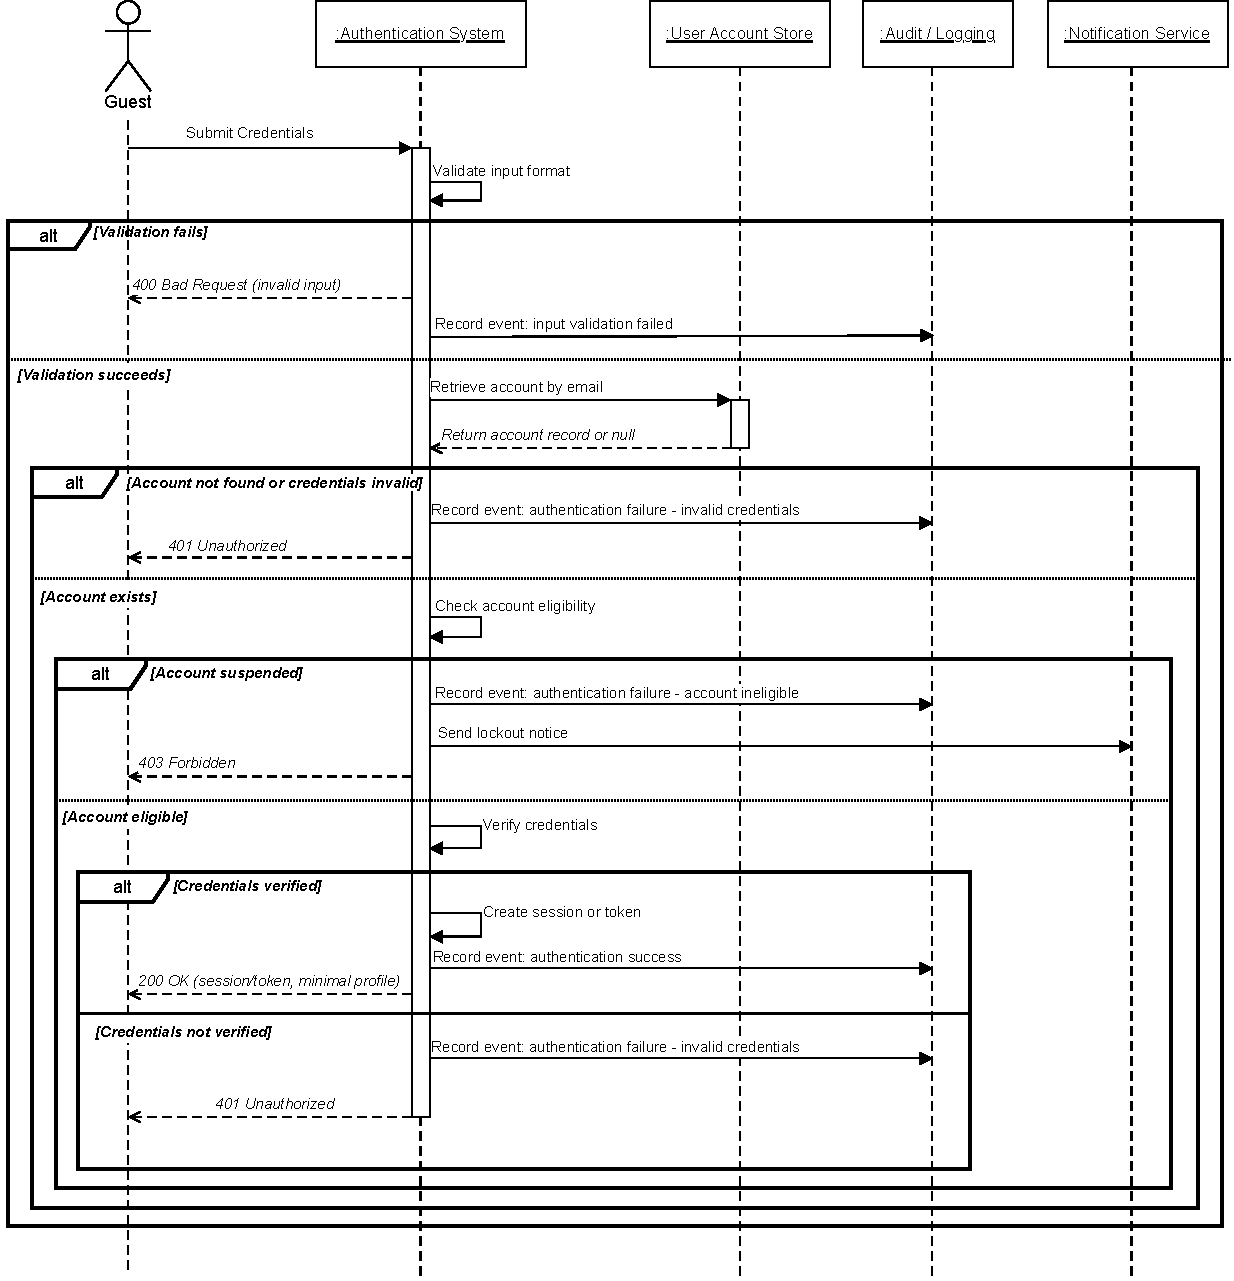
\includegraphics[width=\textwidth]{assets/chapter2/sequence-user-authentication}
    \caption{Sequence Diagram: User Authentication}
    \label{fig:seq-user-authentication}
\end{figure}





\iffalse
\subsection{Register Account and Login Sequence}
This sequence describes the two primary authentication pathways available to
guests: email-based registration with verification and login, and Google
OAuth-based single sign-on. The registration flow validates input, creates a
pending-verification account, dispatches a verification email, and activates
the account upon confirmation. The login flow validates credentials against
stored hashes, enforces rate limiting, and establishes an authenticated session
with the user's assigned role. Google OAuth provides an alternative pathway
where the account is created or linked automatically through the Google
identity provider.

\begin{enumerate}[topsep=0pt,itemsep=1pt,parsep=0pt,partopsep=0pt]
    \item Guest fills out the registration form with name, email, and password
    \item System validates input and checks for duplicate email
    \item System creates the account in pending verification state
    \item System dispatches a verification email
    \item Guest clicks the verification link to activate the account
    \item Guest logs in with email and password or Google OAuth
    \item System validates credentials and creates an authenticated session
    \item System redirects the guest to their role-specific dashboard
\end{enumerate}

Figure~\ref{fig:seq-register-login} illustrates the register account and login
sequence, showing both the email-based registration with verification and the
Google OAuth login pathway.

\begin{figure}[H]
    \centering
    
\includegraphics[width=0.95\textwidth]{assets/chapter2/iot-reap-sequence-register-login.png}
    \caption{Sequence Diagram: Register Account and Login}
    \label{fig:seq-register-login}
\end{figure}

\subsection{Remote Desktop Access Sequence}
This sequence models the connection workflow when an engineer accesses a
provisioned VM session through the Apache Guacamole remote desktop gateway. The
process involves session validation, one-time token generation, Guacamole
connection creation, and the establishment of a live remote desktop session.
The sequence also covers session monitoring and the extension workflow when the
session is about to expire.

\begin{enumerate}[topsep=0pt,itemsep=1pt,parsep=0pt,partopsep=0pt]
    \item Engineer clicks the Connect button on an active VM session
    \item System validates the session status and VM availability
    \item System requests a one-time Guacamole connection token
    \item Guacamole creates the connection with protocol-specific parameters
    \item Frontend opens the Guacamole client in an embedded iframe
    \item Engineer interacts with the remote desktop via keyboard and mouse
    \item System monitors connection health and session timer
    \item If the session is about to expire, the engineer may extend it
\end{enumerate}

Figure~\ref{fig:seq-remote-desktop} presents the remote desktop access
sequence, showing the interaction between the engineer, the frontend, the VM
session service, and the Guacamole gateway.

\begin{figure}[H]
    \centering
    
\includegraphics[width=0.95\textwidth]{assets/chapter2/iot-reap-sequence-remote-desktop.png}
    \caption{Sequence Diagram: Remote Desktop Access}
    \label{fig:seq-remote-desktop}
\end{figure}

\subsection{Session Management Sequence}
This sequence describes the extend and terminate operations that an engineer
can perform on an active VM session. Extension involves checking quota
availability, updating the session expiry, and rescheduling the cleanup job.
Termination involves shutting down the VM through the Proxmox API, updating the
session status, and releasing all associated resources including hardware
reservations and Guacamole connections.

\begin{enumerate}[topsep=0pt,itemsep=1pt,parsep=0pt,partopsep=0pt]
    \item Engineer views their active VM session details
    \item Engineer selects either Extend Session or Terminate Session
    \item If extending, the system checks quota availability for the additional duration
    \item System updates the session expiry and reschedules the cleanup job
    \item If terminating, the system shuts down the VM via the Proxmox API
    \item System updates the session status and releases all associated resources
    \item System removes Guacamole connections and releases hardware reservations
\end{enumerate}

Figure~\ref{fig:seq-session-management} illustrates the session management
sequence, showing both the extension and termination workflows.

\begin{figure}[H]
    \centering
    
\includegraphics[width=0.95\textwidth]{assets/chapter2/iot-reap-sequence-session-management.png}
    \caption{Sequence Diagram: Session Management}
    \label{fig:seq-session-management}
\end{figure}

\subsection{Device Reservation Sequence}
This sequence models the reservation workflow for USB devices and cameras from
the hardware pool. The engineer browses available devices, selects one, and
submits a reservation request. The system checks availability, creates the
reservation, and updates the device status. If the device is unavailable, the
engineer may join a waiting queue and receive a notification when the device
becomes available.

\begin{enumerate}[topsep=0pt,itemsep=1pt,parsep=0pt,partopsep=0pt]
    \item Engineer navigates to the hardware inventory from their session page
    \item System displays available devices with type, model, and status
    \item Engineer selects a device and clicks Reserve
    \item System checks device availability and session compatibility
    \item System creates a reservation linking the device to the session
    \item If the device is unavailable, the engineer joins the device queue
    \item When the device becomes available, the system notifies the next user in queue
\end{enumerate}

Figure~\ref{fig:seq-device-reservation} presents the device reservation
sequence, including the queueing mechanism for unavailable devices.

\begin{figure}[H]
    \centering
    
\includegraphics[width=0.95\textwidth]{assets/chapter2/iot-reap-sequence-device-reservation.png}
    \caption{Sequence Diagram: Device Reservation}
    \label{fig:seq-device-reservation}
\end{figure}

\subsection{Hardware Attach and Detach Sequence}
This sequence describes the attachment and detachment of reserved hardware
devices to a VM session. The attachment workflow invokes the USB/IP proxy to
connect the device to the Proxmox VM, with retry logic on failure. The
detachment workflow safely disconnects the device, updates its status to
available, and removes the reservation record.

\begin{enumerate}[topsep=0pt,itemsep=1pt,parsep=0pt,partopsep=0pt]
    \item Engineer clicks Attach on a reserved device
    \item System invokes the USB/IP proxy to attach the device to the Proxmox VM
    \item If attachment fails, the system retries up to three times
    \item System updates the device status to Attached
    \item Engineer verifies the device appears in the remote desktop
    \item To detach, the engineer clicks Detach on an attached device
    \item System safely disconnects the device via the proxy
    \item System updates the device status to Available and removes the reservation
\end{enumerate}

Figure~\ref{fig:seq-hardware-attach-detach} illustrates the hardware attach and
detach sequence, showing both the attachment and detachment workflows with
error handling.

\begin{figure}[H]
    \centering
    
\includegraphics[width=0.95\textwidth]{assets/chapter2/iot-reap-sequence-hardware-attach-detach.png}
    \caption{Sequence Diagram: Hardware Attach and Detach}
    \label{fig:seq-hardware-attach-detach}
\end{figure}

\subsection{Refund Request Sequence}
This sequence models the engineer-initiated refund request workflow. The
engineer navigates to their payment history, selects a completed payment, and
submits a refund request with a reason. The system validates that the payment
exists, belongs to the requesting user, is within the refund window, and has no
existing refund. Upon successful validation, a refund request is created with
pending status and administrators are notified for review.

\begin{enumerate}[topsep=0pt,itemsep=1pt,parsep=0pt,partopsep=0pt]
    \item Engineer navigates to their payment history
    \item Engineer selects a completed payment and clicks Request Refund
    \item System validates the payment exists and belongs to the user
    \item System checks the refund window has not expired
    \item System checks no duplicate refund exists for this payment
    \item System creates a refund request with pending status
    \item System notifies administrators of the new refund request
    \item Engineer receives confirmation that the request is under review
\end{enumerate}

Figure~\ref{fig:seq-refund-request} presents the refund request sequence,
showing the validation steps and the creation of the pending refund request.

\begin{figure}[H]
    \centering
    
\includegraphics[width=0.95\textwidth]{assets/chapter2/iot-reap-sequence-refund-request.png}
    \caption{Sequence Diagram: Refund Request}
    \label{fig:seq-refund-request}
\end{figure}
\begin{figure}[H]
    \centering
    
\includegraphics[width=\textwidth]{assets/chapter2/iot-reap-sequence-search-training-paths.png}
    \caption{Sequence Diagram: Search Training Paths}
    \label{fig:seq-search-training-paths}
\end{figure}
\begin{figure}[H]
    \centering
    
\includegraphics[width=\textwidth]{assets/chapter2/iot-reap-sequence-activity-logs.png}
    \caption{Sequence Diagram: Activity Logs}
    \label{fig:seq-activity-logs}
\end{figure}
\begin{figure}[H]
    \centering
    
\includegraphics[width=\textwidth]{assets/chapter2/iot-reap-sequence-vm-reservation-approval.png}
    \caption{Sequence Diagram: VM Reservation Approval}
    \label{fig:seq-vm-reservation-approval}
\end{figure}

\subsection{Landing Page Sequence}
This sequence models the guest landing page workflow. The guest navigates to
the home page, the system retrieves featured training paths, and displays them
with course previews. The landing page serves as the primary entry point for
unauthenticated users to discover available learning content.

\begin{enumerate}[topsep=0pt,itemsep=1pt,parsep=0pt,partopsep=0pt]
    \item Guest navigates to the home page
    \item System retrieves featured training paths (limit 3)
    \item System checks registration availability
    \item System renders welcome page with featured courses
    \item Guest views course previews and navigation options
\end{enumerate}

% [FIGURE COMMENTED OUT: Missing image file iot-reap-sequence-landing-page.png]
% Figure~\ref{fig:seq-landing-page} presents the landing page sequence, showing the data retrieval and rendering process for the home page.
%
% \begin{figure}[H]
%     \centering
%     \includegraphics[width=0.95\textwidth]{assets/chapter2/iot-reap-sequence-landing-page.png}
%     \caption{Sequence Diagram: Landing Page}
%     \label{fig:seq-landing-page}
% \end{figure}

\subsection{Legal Pages Sequence}
This sequence models the guest access to legal pages. The guest navigates to
Terms of Service or Privacy Policy pages, the system renders the static
content, and displays the legal documents. These pages are publicly accessible
and require no authentication.

\begin{enumerate}[topsep=0pt,itemsep=1pt,parsep=0pt,partopsep=0pt]
    \item Guest navigates to Terms of Service or Privacy Policy
    \item System retrieves the latest version of the legal document
    \item System renders the document in readable format
    \item Guest views the legal content
\end{enumerate}

% [FIGURE COMMENTED OUT: Missing image file iot-reap-sequence-legal-pages.png]
% Figure~\ref{fig:seq-legal-pages} presents the legal pages sequence, showing the static content rendering process.
%
% \begin{figure}[H]
%     \centering
%     \includegraphics[width=0.95\textwidth]{assets/chapter2/iot-reap-sequence-legal-pages.png}
%     \caption{Sequence Diagram: Legal Pages}
%     \label{fig:seq-legal-pages}
% \end{figure}

\subsection{Password Reset Sequence}
This sequence models the password reset workflow. The user requests a password
reset, the system validates the email, creates a reset token, sends an email
with a secure link, and allows the user to set a new password. The process
includes security measures to prevent email enumeration.

\begin{enumerate}[topsep=0pt,itemsep=1pt,parsep=0pt,partopsep=0pt]
    \item User clicks "Forgot Password" on login page
    \item User enters their email address
    \item System validates the email and creates a reset token
    \item System sends a password reset email with a secure link
    \item User clicks the link and is redirected to the reset form
    \item User enters and confirms a new password
    \item System validates the password and updates the account
    \item System invalidates the reset token and notifies the user
\end{enumerate}

% [FIGURE COMMENTED OUT: Missing image file iot-reap-sequence-password-reset.png]
% Figure~\ref{fig:seq-password-reset} presents the password reset sequence, showing the token generation and password update process.
%
% \begin{figure}[H]
%     \centering
%     \includegraphics[width=0.95\textwidth]{assets/chapter2/iot-reap-sequence-password-reset.png}
%     \caption{Sequence Diagram: Password Reset}
%     \label{fig:seq-password-reset}
% \end{figure}

\subsection{Certificate Verification and Download Sequence}
This sequence models the public certificate verification and download workflow.
A guest or employer verifies a certificate using its hash, the system validates
the hash, retrieves the certificate details, and allows PDF download. This
enables third-party verification of course completion.

\begin{enumerate}[topsep=0pt,itemsep=1pt,parsep=0pt,partopsep=0pt]
    \item Guest receives a certificate (via email or LinkedIn)
    \item Guest navigates to the certificate verification page
    \item Guest enters the certificate hash or clicks a verification link
    \item System validates the hash and retrieves the certificate record
    \item System displays certificate details (engineer, course, completion date)
    \item Guest clicks download certificate
    \item System generates PDF and triggers file download
\end{enumerate}

% [FIGURE COMMENTED OUT: Missing image file iot-reap-sequence-certificate-verification.png]
% Figure~\ref{fig:seq-certificate-verification} presents the certificate verification sequence, showing the hash validation and PDF generation process.
%
% \begin{figure}[H]
%     \centering
%     \includegraphics[width=0.95\textwidth]{assets/chapter2/iot-reap-sequence-certificate-verification.png}
%     \caption{Sequence Diagram: Certificate Verification and Download}
%     \label{fig:seq-certificate-verification}
% \end{figure}

\subsection{Checkout Result Screens Sequence}
This sequence models the checkout result page workflows. After completing or
cancelling payment on Stripe, the user is redirected to success or cancellation
pages. The system retrieves the session details, updates enrollment status, and
displays appropriate result screens with next steps.

\begin{enumerate}[topsep=0pt,itemsep=1pt,parsep=0pt,partopsep=0pt]
    \item User completes payment on Stripe
    \item Stripe redirects to success or cancellation page
    \item System retrieves checkout session details
    \item System validates the session and updates enrollment status
    \item System renders success page with course access
    \item Or system renders cancellation page with retry options
\end{enumerate}

% [FIGURE COMMENTED OUT: Missing image file iot-reap-sequence-checkout-result.png]
% Figure~\ref{fig:seq-checkout-result} presents the checkout result screens sequence, showing the redirect handling and status updates.

\subsection{VM Snapshots Sequence}
This sequence models the VM snapshot viewing workflow. The engineer views
available snapshots for a session or browses Proxmox VM snapshots across
servers. The system queries Proxmox for snapshot lists and displays them with
metadata for session provisioning context.

\begin{enumerate}[topsep=0pt,itemsep=1pt,parsep=0pt,partopsep=0pt]
    \item Engineer opens the sessions interface
    \item Engineer selects a session and views snapshots
    \item System queries Proxmox for VM snapshots
    \item System displays snapshots with names and timestamps
    \item Or engineer browses Proxmox VM browser
    \item System displays available VMs and their snapshots
\end{enumerate}

% [FIGURE COMMENTED OUT: Missing image file iot-reap-sequence-vm-snapshots.png]
% Figure~\ref{fig:seq-vm-snapshots} presents the VM snapshots sequence, showing the Proxmox integration and snapshot display.

\subsection{Hardware Inventory and Status Sequence}
This sequence models the hardware inventory viewing workflow. The engineer
browses available USB devices and cameras, checks their status, and refreshes
device information. The system queries gateway nodes for real-time device
status and displays the inventory with availability information.

\begin{enumerate}[topsep=0pt,itemsep=1pt,parsep=0pt,partopsep=0pt]
    \item Engineer navigates to hardware inventory page
    \item System retrieves gateway nodes and device lists
    \item System queries device status from gateways
    \item System displays devices with status (available, reserved, maintenance)
    \item Engineer clicks refresh to update device status
    \item System re-queries gateways and updates display
\end{enumerate}

% [FIGURE COMMENTED OUT: Missing image file iot-reap-sequence-hardware-inventory.png]
% Figure~\ref{fig:seq-hardware-inventory} presents the hardware inventory sequence, showing the gateway integration and status monitoring.

\subsection{Camera Management Extras Sequence}
This sequence models the advanced camera management workflow. The engineer
views camera streams, acquires PTZ control, adjusts resolution, and manages
WebRTC streaming. The system handles camera control locking, stream quality
optimization, and real-time video delivery.

\begin{enumerate}[topsep=0pt,itemsep=1pt,parsep=0pt,partopsep=0pt]
    \item Engineer views session cameras
    \item Engineer selects camera and views stream
    \item Engineer acquires PTZ control
    \item System grants control and enables PTZ commands
    \item Engineer sends PTZ move commands
    \item Engineer adjusts stream resolution
    \item System starts WebRTC stream (WHEP)
    \item Engineer releases camera control
\end{enumerate}

% [FIGURE COMMENTED OUT: Missing image file iot-reap-sequence-camera-management-extras.png]
% Figure~\ref{fig:seq-camera-management-extras} presents the camera management extras sequence, showing PTZ control and streaming management.

\subsection{VM Reservation Sequence}
This sequence models the VM reservation workflow. The engineer browses
available VMs, views reservation calendars, creates time-based reservations,
and manages reservation status. The system checks for conflicts, creates
reservation records, and handles approval workflows.

\begin{enumerate}[topsep=0pt,itemsep=1pt,parsep=0pt,partopsep=0pt]
    \item Engineer views available VMs
    \item Engineer selects VM and views reservation calendar
    \item Engineer selects time slot and creates reservation
    \item System checks for conflicting reservations
    \item System creates reservation with pending status
    \item Engineer views reservation details and status
    \item Engineer cancels reservation if needed
\end{enumerate}

% [FIGURE COMMENTED OUT: Missing image file iot-reap-sequence-vm-reservation.png]
% Figure~\ref{fig:seq-vm-reservation} presents the VM reservation sequence, showing the conflict detection and reservation management.

\subsection{Learning Content Sequence}
This sequence models the learning content consumption workflow. The engineer
enrolls in training paths, watches videos, reads articles, takes quizzes, and
tracks progress. The system records completion status, updates progress
indicators, and manages learning state across different content types.

\begin{enumerate}[topsep=0pt,itemsep=1pt,parsep=0pt,partopsep=0pt]
    \item Engineer views enrolled training paths
    \item Engineer selects training path and views modules
    \item Engineer watches video lesson
    \item System records video progress and updates completion
    \item Engineer reads article lesson
    \item System marks article as read and updates progress
    \item Engineer takes quiz assessment
    \item System evaluates answers and records score
    \item Engineer marks unit as complete
    \item System recalculates overall path progress
\end{enumerate}

% [FIGURE COMMENTED OUT: Missing image file iot-reap-sequence-learning-content.png]
% Figure~\ref{fig:seq-learning-content} presents the learning content sequence, showing the progress tracking across different content types.

\subsection{Training Path Authoring Sequence}
This sequence models the training path creation workflow. The teacher creates
training paths, adds modules and units, organizes content structure, and
submits for review. The system manages the hierarchical content structure,
validates completeness, and handles the approval workflow.

\begin{enumerate}[topsep=0pt,itemsep=1pt,parsep=0pt,partopsep=0pt]
    \item Teacher navigates to teaching workspace
    \item Teacher creates new training path
    \item Teacher adds modules to the path
    \item Teacher adds training units to modules
    \item Teacher reorders modules and units
    \item Teacher edits path details and content
    \item Teacher submits path for admin review
    \item System updates status to pending\_review
    \item Teacher can archive or delete paths
\end{enumerate}

% [FIGURE COMMENTED OUT: Missing image file iot-reap-sequence-training-path-authoring.png]
% Figure~\ref{fig:seq-training-path-authoring} presents the training path authoring sequence, showing the hierarchical content management.

\subsection{Teacher Content Flows Sequence}
This sequence models the content authoring workflows for teachers. The teacher
creates quizzes, writes articles, uploads videos, manages captions, and
publishes content. The system handles content processing, status management,
and quality control for different content types.

\begin{enumerate}[topsep=0pt,itemsep=1pt,parsep=0pt,partopsep=0pt]
    \item Teacher creates quiz with questions
    \item Teacher publishes or unpublishes quiz
    \item Teacher views quiz statistics
    \item Teacher writes article content
    \item Teacher updates or deletes article
    \item Teacher uploads video file
    \item System processes video asynchronously
    \item Teacher checks processing status
    \item Teacher retries failed processing
    \item Teacher manages video captions
    \item Teacher deletes video and captions
\end{enumerate}

% [FIGURE COMMENTED OUT: Missing image file iot-reap-sequence-teacher-content-flows.png]
% Figure~\ref{fig:seq-teacher-content-flows} presents the teacher content flows sequence, showing the content management for different types.

\subsection{Teacher Forum Moderation Sequence}
This sequence models the teacher forum moderation workflow. The teacher views
forum inbox, pins important threads, locks discussions, marks answers, and
manages community interactions. The system handles moderation actions,
notifications, and thread management for course discussions.

\begin{enumerate}[topsep=0pt,itemsep=1pt,parsep=0pt,partopsep=0pt]
    \item Teacher navigates to forum inbox
    \item Teacher views threads and replies for their courses
    \item Teacher pins or unpins important threads
    \item Teacher locks or unlocks discussions
    \item Teacher marks reply as accepted answer
    \item Teacher resolves flagged content
    \item Teacher posts replies and upvotes content
    \item Teacher flags inappropriate content
\end{enumerate}

% [FIGURE COMMENTED OUT: Missing image file iot-reap-sequence-teacher-forum-moderation.png]
% Figure~\ref{fig:seq-teacher-forum-moderation} presents the teacher forum moderation sequence, showing the community management capabilities.

\subsection{Teacher Analytics and Payouts Sequence}
This sequence models the teacher analytics and payout workflows. The teacher
views performance metrics, tracks earnings, requests payouts, and exports
reports. The system calculates KPIs, manages payout requests, and handles
financial transactions for instructors.

\begin{enumerate}[topsep=0pt,itemsep=1pt,parsep=0pt,partopsep=0pt]
    \item Teacher views analytics dashboard
    \item Teacher views KPIs (engineers, revenue, completion)
    \item Teacher views enrollment and revenue charts
    \item Teacher views engineer progress per course
    \item Teacher views completion funnel
    \item Teacher views earnings summary
    \item Teacher requests payout
    \item Teacher exports earnings report
\end{enumerate}

% [FIGURE COMMENTED OUT: Missing image file iot-reap-sequence-teacher-analytics-payouts.png]
% Figure~\ref{fig:seq-teacher-analytics-payouts} presents the teacher analytics and payouts sequence, showing the performance tracking and financial management.

\subsection{Teacher VM Assignments Sequence}
This sequence models the VM assignment workflow for teachers. The teacher
browses available VM templates, submits assignments for training units, and
manages assignment status. The system handles the approval workflow, VM
assignment tracking, and integration with course content.

\begin{enumerate}[topsep=0pt,itemsep=1pt,parsep=0pt,partopsep=0pt]
    \item Teacher views available VM templates
    \item Teacher selects training unit for VM assignment
    \item Teacher checks existing VM assignment
    \item Teacher submits VM assignment
    \item System creates assignment with pending\_approval status
    \item Teacher views assignment details and status
    \item Teacher updates or deletes assignment
\end{enumerate}

% [FIGURE COMMENTED OUT: Missing image file iot-reap-sequence-teacher-vm-assignments.png]
% Figure~\ref{fig:seq-teacher-vm-assignments} presents the teacher VM assignments sequence, showing the assignment submission and approval workflow.

\subsection{Admin Dashboard and KPIs Sequence}
This sequence models the admin dashboard and KPI viewing workflow. The
administrator views platform metrics, checks system health, monitors alerts,
and reviews activity logs. The system aggregates data from multiple sources and
provides real-time visibility into platform performance.

\begin{enumerate}[topsep=0pt,itemsep=1pt,parsep=0pt,partopsep=0pt]
    \item Administrator navigates to admin dashboard
    \item System displays platform KPIs (users, revenue, sessions)
    \item Administrator views system health indicators
    \item Administrator views system alerts
    \item Administrator views activity logs
    \item Administrator filters logs by user or date range
    \item Administrator views activity statistics
\end{enumerate}

% [FIGURE COMMENTED OUT: Missing image file iot-reap-sequence-admin-dashboard-kpis.png]
% Figure~\ref{fig:seq-admin-dashboard-kpis} presents the admin dashboard and KPIs sequence, showing the platform monitoring and analytics.

\subsection{Admin Alerts Sequence}
This sequence models the system alerts management workflow. The administrator
views alerts, acknowledges issues, resolves problems, and manages alert
lifecycle. The system handles alert generation, status tracking, and
notification management for platform monitoring.

\begin{enumerate}[topsep=0pt,itemsep=1pt,parsep=0pt,partopsep=0pt]
    \item Administrator views system alerts
    \item Administrator views unacknowledged alerts
    \item Administrator views alert statistics
    \item Administrator acknowledges individual alert
    \item Administrator acknowledges all alerts
    \item Administrator resolves alert with notes
    \item Administrator deletes old alerts
\end{enumerate}

% [FIGURE COMMENTED OUT: Missing image file iot-reap-sequence-admin-alerts.png]
% Figure~\ref{fig:seq-admin-alerts} presents the admin alerts sequence, showing the alert management and resolution workflow.

\subsection{Admin User Governance Sequence}
This sequence models the user management workflow for administrators. The admin
views users, approves teachers, manages roles, suspends accounts, and handles
compliance actions. The system enforces role-based access, manages user
lifecycle, and maintains security governance.

\begin{enumerate}[topsep=0pt,itemsep=1pt,parsep=0pt,partopsep=0pt]
    \item Administrator views all users
    \item Administrator views user details
    \item Administrator approves teacher account
    \item Administrator revokes teacher approval
    \item Administrator suspends user account
    \item Administrator unsuspends user account
    \item Administrator changes user role
    \item Administrator impersonates user for debugging
    \item Administrator performs data deletion
\end{enumerate}

% [FIGURE COMMENTED OUT: Missing image file iot-reap-sequence-admin-user-governance.png]
% Figure~\ref{fig:seq-admin-user-governance} presents the admin user governance sequence, showing the user management and security actions.

\subsection{Admin Infrastructure Sequence}
This sequence models the infrastructure management workflow. The administrator
manages Proxmox servers, controls VMs, manages hardware gateways, and monitors
system resources. The system handles server connectivity, VM lifecycle,
hardware discovery, and infrastructure health monitoring.

\begin{enumerate}[topsep=0pt,itemsep=1pt,parsep=0pt,partopsep=0pt]
    \item Administrator views Proxmox servers
    \item Administrator tests server connection
    \item Administrator registers new server
    \item Administrator edits server credentials
    \item Administrator inactivates or deletes server
    \item Administrator syncs nodes from server
    \item Administrator manages VMs (start, stop, reboot)
    \item Administrator manages gateway nodes
    \item Administrator discovers hardware devices
    \item Administrator refreshes gateway status
\end{enumerate}

% [FIGURE COMMENTED OUT: Missing image file iot-reap-sequence-admin-infrastructure.png]
% Figure~\ref{fig:seq-admin-infrastructure} presents the admin infrastructure sequence, showing the comprehensive infrastructure management.

\subsection{Admin Camera and Reservation Administration Sequence}
This sequence models the camera and reservation administration workflow. The
administrator manages camera assignments, approves reservations, blocks time
slots, and oversees resource allocation. The system handles camera-VM
associations, reservation approval workflows, and resource availability
management.

\begin{enumerate}[topsep=0pt,itemsep=1pt,parsep=0pt,partopsep=0pt]
    \item Administrator views all cameras
    \item Administrator assigns camera to VM
    \item Administrator unassigns camera
    \item Administrator bulk assigns cameras
    \item Administrator activates or deactivates camera
    \item Administrator views USB reservations
    \item Administrator approves or rejects USB reservation
    \item Administrator blocks device time slot
    \item Administrator views camera reservations
    \item Administrator approves or rejects camera reservation
\end{enumerate}

% [FIGURE COMMENTED OUT: Missing image file iot-reap-sequence-admin-camera-reservation.png]
% Figure~\ref{fig:seq-admin-camera-reservation} presents the admin camera and reservation administration sequence, showing the resource management workflows.

\subsection{Admin Finance Sequence}
This sequence models the financial management workflow for administrators. The
admin manages payouts, processes refunds, reviews financial transactions, and
handles Stripe integration. The system validates financial requests, executes
transfers, maintains audit trails, and ensures transaction integrity.

\begin{enumerate}[topsep=0pt,itemsep=1pt,parsep=0pt,partopsep=0pt]
    \item Administrator views finance overview
    \item Administrator views payout requests
    \item Administrator exports payouts report
    \item Administrator approves payout request
    \item Administrator rejects payout request
    \item Administrator processes payout transfer via Stripe
    \item Administrator views refund requests
    \item Administrator views all refunds history
    \item Administrator approves refund request
    \item Administrator executes Stripe refund
    \item Administrator rejects refund request
\end{enumerate}

% [FIGURE COMMENTED OUT: Missing image file iot-reap-sequence-admin-finance.png]
% Figure~\ref{fig:seq-admin-finance} presents the admin finance sequence, showing the financial transaction management and Stripe integration.

\subsection{Admin Maintenance Sequence}
This sequence models the maintenance management workflow. The administrator
places devices in maintenance mode, sets maintenance descriptions, and manages
device availability. The system handles maintenance status updates, gateway
integration, and prevents reservations during maintenance periods.

\begin{enumerate}[topsep=0pt,itemsep=1pt,parsep=0pt,partopsep=0pt]
    \item Administrator views devices in maintenance
    \item Administrator sets USB device maintenance description
    \item Administrator enables USB device maintenance
    \item Administrator disables USB device maintenance
    \item Administrator enables camera maintenance mode
    \item Administrator disables camera maintenance mode
\end{enumerate}

% [FIGURE COMMENTED OUT: Missing image file iot-reap-sequence-admin-maintenance.png]
% Figure~\ref{fig:seq-admin-maintenance} presents the admin maintenance sequence, showing the device maintenance management.

\subsection{Admin Moderation and Video Monitor Sequence}
This sequence models the content moderation and video monitoring workflow. The
administrator reviews flagged forum content, takes moderation actions, monitors
camera streams, and manages video recordings. The system handles content
review, user notifications, and real-time video monitoring.

\begin{enumerate}[topsep=0pt,itemsep=1pt,parsep=0pt,partopsep=0pt]
    \item Administrator views flagged forum threads
    \item Administrator views flagged replies
    \item Administrator reviews thread content
    \item Administrator unflags thread or reply
    \item Administrator deletes inappropriate content
    \item Administrator views active camera streams
    \item Administrator monitors specific camera
    \item Administrator takes PTZ control
    \item Administrator views camera recordings
    \item Administrator downloads recording
    \item Administrator views camera analytics
\end{enumerate}

% [FIGURE COMMENTED OUT: Missing image file iot-reap-sequence-admin-moderation-video-monitor.png]
% Figure~\ref{fig:seq-admin-moderation-video-monitor} presents the admin moderation and video monitor sequence, showing the content moderation and surveillance capabilities.

\subsection{Stripe Checkout Sequence}
This sequence models the Stripe checkout payment workflow. The user initiates
checkout, the system creates a Stripe session, redirects to payment, and
handles the result. The system manages enrollment creation, payment
confirmation, and webhook processing for transaction completion.

\begin{enumerate}[topsep=0pt,itemsep=1pt,parsep=0pt,partopsep=0pt]
    \item User views training path details
    \item User clicks enroll or purchase
    \item System creates pending enrollment
    \item System creates Stripe Checkout session
    \item System redirects user to Stripe payment
    \item User completes payment on Stripe
    \item Stripe redirects to success or cancellation page
    \item System updates enrollment status
    \item System creates payment record
    \item System notifies user and teacher
\end{enumerate}

% [FIGURE COMMENTED OUT: Missing image file iot-reap-sequence-stripe-checkout.png]
% Figure~\ref{fig:seq-stripe-checkout} presents the Stripe checkout sequence, showing the payment integration and enrollment activation.

\subsection{Stripe Refund Sequence}
This sequence models the Stripe refund workflow. The user requests a refund,
the admin approves the request, and the system executes the refund through
Stripe. The system handles refund eligibility checking, approval workflows,
Stripe integration, and enrollment revocation.

\begin{enumerate}[topsep=0pt,itemsep=1pt,parsep=0pt,partopsep=0pt]
    \item User views enrolled courses
    \item User requests refund with reason
    \item System validates refund eligibility
    \item System creates refund request with pending status
    \item System notifies admins
    \item Administrator reviews refund request
    \item Administrator approves or rejects request
    \item System executes Stripe refund if approved
    \item System updates payment and enrollment status
    \item System notifies user and teacher
\end{enumerate}

% [FIGURE COMMENTED OUT: Missing image file iot-reap-sequence-stripe-refund.png]
% Figure~\ref{fig:seq-stripe-refund} presents the Stripe refund sequence, showing the refund request and execution workflow.

\subsection{Stripe Payout Sequence}
This sequence models the Stripe payout workflow for instructors. The teacher
requests payout, the admin approves the request, and the system processes the
transfer through Stripe. The system handles earnings validation, payout
management, Stripe transfer execution, and teacher notifications.

\begin{enumerate}[topsep=0pt,itemsep=1pt,parsep=0pt,partopsep=0pt]
    \item Teacher views earnings summary
    \item Teacher requests payout
    \item System validates available balance
    \item System creates payout request with pending status
    \item System deducts from available balance
    \item System notifies admins
    \item Administrator reviews payout request
    \item Administrator approves or rejects request
    \item System processes Stripe transfer if approved
    \item System updates payout status to paid
    \item System notifies teacher of completion
\end{enumerate}

% [FIGURE COMMENTED OUT: Missing image file iot-reap-sequence-stripe-payout.png]
% Figure~\ref{fig:seq-stripe-payout} presents the Stripe payout sequence, showing the instructor payout and transfer workflow.

\subsection{Stripe Webhooks Sequence}
This sequence models the Stripe webhook processing workflow. Stripe sends
webhook events for payment status changes, the system verifies signatures,
processes events, and updates internal records. The system handles multiple
event types, ensures idempotency, and maintains transaction integrity.

\begin{enumerate}[topsep=0pt,itemsep=1pt,parsep=0pt,partopsep=0pt]
    \item Stripe sends webhook event
    \item System verifies webhook signature
    \item System parses event type and data
    \item System processes checkout.session.completed event
    \item System processes payment\_intent.succeeded event
    \item System processes payment\_intent.payment\_failed event
    \item System processes charge.refunded event
    \item System processes transfer.created event
    \item System processes transfer.paid event
    \item System processes transfer.failed event
    \item System updates internal records
    \item System notifies relevant users
\end{enumerate}

% [FIGURE COMMENTED OUT: Missing image file iot-reap-sequence-stripe-webhooks.png]
% Figure~\ref{fig:seq-stripe-webhooks} presents the Stripe webhooks sequence, showing the event processing and system integration.
\iffalse
    \subsubsection*{Activity Diagrams}

    The activity diagrams below complement the sequence diagrams by emphasizing
    decisions, branch conditions, and process states. In this platform, they are
    especially useful for approval workflows and infrastructure-dependent
    operations where multiple outcomes are possible.

    \subsection{Training Path Approval Activity}

    The activity starts with a teacher submission and ends either with approval or
    rejection. The major states are content preparation, submission, administrative
    review, decision, and post-decision visibility. If the administrator approves
    the path, it becomes available in the approved catalog and may later be
    featured. If rejected, the path returns to the teacher for revision.
    Figure~\ref{fig:act-tp-approval} presents the training path approval activity
    diagram, showing the decision branches between approval and rejection.

    \begin{figure}[H]
        \centering
        
\includegraphics[width=0.85\textwidth]{assets/chapter2/iot-reap-activity-tp-approval.png}
        \caption{Activity Diagram: Training Path Approval}
        \label{fig:act-tp-approval}
    \end{figure}

    \subsection{Virtual Machine Session Lifecycle Activity}

    The VM lifecycle activity begins with a session request and progresses through
    authorization, capacity verification, session creation, active usage, extension
    or expiration, and termination. A failure branch exists whenever no capacity is
    available or provisioning fails. A normal branch leads to active session
    access, optional snapshot consultation, remote connection token generation, and
    eventual cleanup. Figure~\ref{fig:act-vm-lifecycle} presents the virtual
    machine session lifecycle activity diagram, including the failure branch and
    the normal operational flow.

    \begin{figure}[H]
        \centering
        
\includegraphics[width=0.85\textwidth]{assets/chapter2/iot-reap-activity-vm-lifecycle.png}
        \caption{Activity Diagram: Virtual Machine Session Lifecycle}
        \label{fig:act-vm-lifecycle}
    \end{figure}

    \subsection{Reservation Management Activity}

    Reservation activity applies to USB devices and cameras. The process begins
    with calendar consultation, followed by request submission, conflict
    verification, pending review, approval or rejection, activation within the
    scheduled period, and completion or cancellation. Administrative intervention
    may also insert blocked periods or maintenance-driven unavailability.
    Figure~\ref{fig:act-reservation} presents the reservation management activity
    diagram, showing the flow from consultation through approval or rejection to
    activation and completion.

    \begin{figure}[H]
        \centering
        
\includegraphics[width=0.85\textwidth]{assets/chapter2/iot-reap-activity-reservation.png}
        \caption{Activity Diagram: Reservation Management}
        \label{fig:act-reservation}
    \end{figure}

    \subsection{Refund Processing Activity}

    The refund process begins when an engineer submits a refund request for a
    payment. The request enters a pending state, is reviewed by an administrator,
    and either gets approved or rejected. If approved, the process continues to
    refund execution and final completion; if rejected, the request is closed with
    explanatory notes. This activity illustrates how payment governance is handled
    as an auditable business workflow rather than a simple transaction update.
    Figure~\ref{fig:act-refund} presents the refund processing activity diagram,
    showing the decision branches between approval and rejection and the subsequent
    execution or closure.

    \begin{figure}[H]
        \centering
        
\includegraphics[width=0.85\textwidth]{assets/chapter2/iot-reap-activity-refund.png}
        \caption{Activity Diagram: Refund Processing}
        \label{fig:act-refund}
    \end{figure}

    \subsection{Account Registration Activity}

    The account registration activity covers the user onboarding workflow from the
    initial registration form through email verification and optional role
    selection. The process begins when a guest fills out the registration form with
    name, email, and password. The system validates the input, creates the user
    account in an unverified state, and dispatches a verification email. The user
    must click the verification link to activate the account. For accounts created
    through Google OAuth, the email is pre-verified and the user is prompted to
    select a role. If the user chooses the teacher role, the account enters a
    pending approval state until an administrator grants teacher privileges.
    Figure~\ref{fig:act-registration} presents the account registration activity
    diagram, including the email verification branch and the role selection
    decision.

    \begin{figure}[H]
        \centering
        
\includegraphics[width=0.85\textwidth]{assets/chapter2/iot-reap-activity-registration.png}
        \caption{Activity Diagram: Account Registration}
        \label{fig:act-registration}
    \end{figure}

    \subsection{Supplementary Activity Diagrams}

    The following activity diagrams provide detailed workflow descriptions for key
    use cases that complement the diagrams presented earlier in this chapter.

    \textbf{Device Reservation.} The device reservation activity diagram illustrates the workflow for reserving a USB device or camera. The engineer selects a device type and preferred time slot, the system checks availability, and upon confirmation the reservation is recorded with a pending status. If the device is already reserved, the engineer may join a wait queue. Figure~\ref{fig:act-device-reservation} presents this workflow.

    \begin{figure}[H]
        \centering
        
\includegraphics[width=0.85\textwidth]{assets/chapter2/iot-reap-activity-device-reservation.png}
        \caption{Activity Diagram: Device Reservation}
        \label{fig:act-device-reservation}
    \end{figure}

    \textbf{Specification of the Use Case Hardware Attach/Detach.} The hardware attach and detach activity diagram shows the process of connecting or disconnecting USB devices from a running virtual machine. The engineer initiates the operation, the system verifies the device status and VM state, performs the USB redirection through the Proxmox agent, and confirms the result. Figure~\ref{fig:act-hardware-attach-detach} presents this workflow.

    \begin{figure}[H]
        \centering
        
\includegraphics[width=0.85\textwidth]{assets/chapter2/iot-reap-activity-hardware-attach-detach.png}
        \caption{Activity Diagram: Hardware Attach/Detach}
        \label{fig:act-hardware-attach-detach}
    \end{figure}

    \textbf{Specification of the Use Case Quiz Attempt.} The quiz attempt activity diagram depicts the workflow when an engineer takes a quiz within a training path. The system loads the quiz questions, the engineer submits answers, each answer is evaluated, and the final score is calculated. If the passing threshold is met, a certificate may be issued. Figure~\ref{fig:act-quiz-attempt} presents this workflow.

    \begin{figure}[H]
        \centering
        
\includegraphics[width=0.85\textwidth]{assets/chapter2/iot-reap-activity-quiz-attempt.png}
        \caption{Activity Diagram: Quiz Attempt}
        \label{fig:act-quiz-attempt}
    \end{figure}

    \textbf{Specification of the Use Case Refund Request.} The refund request activity diagram shows the process when an engineer requests a refund for a training path enrollment. The engineer submits the request with a reason, the system validates the refund policy and eligibility period, and the request is forwarded to an administrator for approval or rejection. Figure~\ref{fig:act-refund-request} presents this workflow.

    \begin{figure}[H]
        \centering
        
\includegraphics[width=0.85\textwidth]{assets/chapter2/iot-reap-activity-refund-request.png}
        \caption{Activity Diagram: Refund Request}
        \label{fig:act-refund-request}
    \end{figure}

    \textbf{Specification of the Use Case Account Registration and Login.} The account registration and login activity diagram covers the combined authentication workflow. It begins with the guest choosing between registration and login, proceeds through form validation and credential verification, handles Google OAuth as an alternative path, and includes email verification and role selection branches. Figure~\ref{fig:act-register-login} presents this workflow.

    \begin{figure}[H]
        \centering
        
\includegraphics[width=0.85\textwidth]{assets/chapter2/iot-reap-activity-register-login.png}
        \caption{Activity Diagram: Account Registration and Login}
        \label{fig:act-register-login}
    \end{figure}

    \textbf{Specification of the Use Case Session Management.} The session management activity diagram illustrates the lifecycle of a VM session from creation through extension and termination. The engineer provisions a session, the system clones the template VM via Proxmox, creates a Guacamole connection, and the engineer can extend or terminate the session. Automatic cleanup occurs when the session expires. Figure~\ref{fig:act-session-management} presents this workflow.

    \begin{figure}[H]
        \centering
        
\includegraphics[width=0.85\textwidth]{assets/chapter2/iot-reap-activity-session-management.png}
        \caption{Activity Diagram: Session Management}
        \label{fig:act-session-management}
    \end{figure}
    \begin{figure}[H]
        \centering
        
\includegraphics[width=\textwidth]{assets/chapter2/iot-reap-activity-forum-moderation.png}
        \caption{Activity Diagram: Forum Moderation}
        \label{fig:act-forum-moderation}
    \end{figure}
    \begin{figure}[H]
        \centering
        
\includegraphics[width=\textwidth]{assets/chapter2/iot-reap-activity-camera-reservation-approval.png}
        \caption{Activity Diagram: Camera Reservation Approval}
        \label{fig:act-camera-reservation-approval}
    \end{figure}
\fi

\fi





